\documentclass[12pt]{fithesis2}

% ===== LOADING PACKAGES =====
% language settings, main documnet language last
\usepackage[english]{babel}
% enabling new fonts support (nicer)
\usepackage{lmodern}
% setting input encoding
\usepackage[utf8]{inputenc}
% setting output encoding
\usepackage[T1]{fontenc}
% fithesis2 requires csquotes
\usepackage{csquotes}

\usepackage{subfig}
\usepackage{graphicx}
\usepackage{kpfonts}
\usepackage[labelfont=bf]{caption}
\usepackage{stmaryrd}

\usepackage[
    backend=biber,      % use biber as backend instead of BiBTeX
    style=alphabetic,   % citation style
	url=true,           % display urls in bibliography
	hyperref=auto,      % detect hyperref and create links
    firstinits=true,    % abbreviate first names to initials
    maxbibnames=5,      % maxiumim number of authors before making 'et al.'
    alldates=iso8601,   % set date format to ISO 8601
]{biblatex}
\addbibresource{thesis.bib}
% setting custom colors for l

% FI THESIS settings
\thesistitle{Something with BCS}
\thesissubtitle{Master thesis}
\thesisstudent{Matej Troják}
\thesiswoman{false}
\thesisfaculty{fi}
\thesisyear{autumn 2017}
\thesisadvisor{RNDr.\ David Šafránek,\ Ph.D.}
\thesislang{en}

% ===== BEGIN DOCUMENT =====
\begin{document}

\FrontMatter
\ThesisTitlePage

\begin{ThesisDeclaration}
\DeclarationText
\AdvisorName
\end{ThesisDeclaration}

\begin{ThesisThanks}
Many thanks to you all.

\vspace{1em}
\noindent
There would be much less
algebra,        % advancements, art, adrenaline, archery, astrophotography, algebra
board gaming,   % beauty, baking, beer, board gaming
curiosity,      % courage, contemplation, cooking, cakes, curiosity
drama,          % discipline, devotion, drama
experience,     % empathy, experience
functional programmig,  % fun, friendliness, faith, functional programmig
geekiness,      % GEB, good books, geekiness
honesty,        % humour, honesty
inspiration,    % improvements, ideas, idealisms, inspiration
joy,            % jokes, joy
knowledge,      % knowledge
learning,       % learning, love
magic,          % meaning, magic, miracles, meta, moose
nighttime walks,    % nighttime walks, Norway
OpenLabs,       % organization, openness, optimism, OpenLabs
puzzle hunts,   % peace, patience, procrastination, puzzle hunts
quiet,          % quiet
respect,        % research, respect
surprises,      % spontaneity, silence, security, stories, star gazing, surprises
trust,          % typographic correctness, tolerance, trust
unpredictability,   % understanding, unity, unpredictability
vigilance,      % vigilance
Wachumba,       % wisdom, Wachumba
xylophone,      % xylophone
yummies         % yellow, you, yummies
and
zeal            % Zendo, Zen, zeal
in the world for me without you.

\vspace{0.65\textheight}
\noindent
Access to computing and storage facilities owned by parties and projects contributing to the National Grid Infrastructure MetaCentrum, provided under the programme Projects of Large Infrastructure for Research, Development, and Innovations(LM2010005), is greatly appreciated.
\end{ThesisThanks}

\begin{ThesisAbstract}
This thesis explores the randomness of outputs created by authenticated encryption schemes submitted to the  competition. Tested scenarios included three different modes of public message numbers. For the assessment, four different software tools were used: three common statistical batteries and a novel genetically inspired framework. The obtained results are interpreted in two ways: Firstly, to gain insights into the quality of the proposed  candidates. Secondly, to compare and contrast the used randomness testing tools. Directions for future research are proposed based on the obtained conclusions.
\end{ThesisAbstract}

\begin{ThesisKeyWords}
statistical randomness, authenticated encryption, CAESAR, evolutionary algorithms, genetic programming
\end{ThesisKeyWords}

\MainMatter
\tableofcontents

\chapter{Introduction}

\chapter{Background}
\section{Rule-based basics}

In our last paper~\cite{Ded201627}, we defined semantics of Biochemical Space Language (BCSL) via translating to a similar language called Kappa~\cite{Kappa}. However, we realised this approach is not very beneficial since we are not fully using the expressive power of our language this way. The thing is Kappa operates purely on expressions. We want to promote our language to a higher level when it operates on objects in multisets. By translating to Kappa we loose such abstraction. 

The reason for this kind of abstraction is the way how we see the biological models. We represent model $\mathcal{M}$ as set of rules and an initial solution of interacting entities. We understand solution as a mixture of individual objects which are randomly distributed (see Fig.~\ref{solutions:fig}a). Therefore, we cannot assign them any order and we do not see them as expressions but rather as multisets. For us, this representation of solution is the closest to the reality.

\begin{figure}
\begin{center}
\subfloat[]{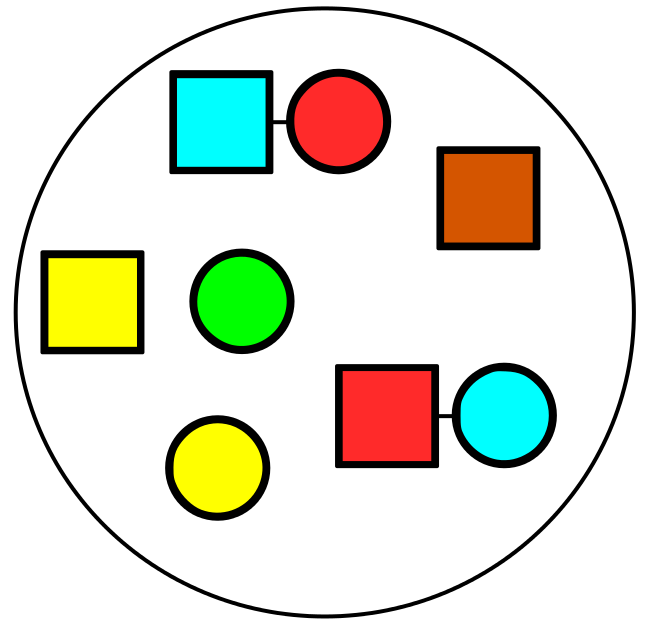
\includegraphics[scale=0.23]{solution_first}\label{sol:s1}}
\hspace*{1cm}
\subfloat[]{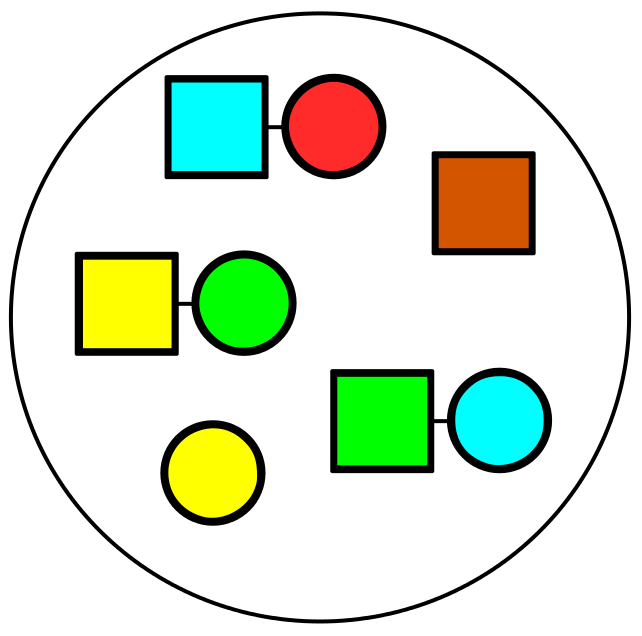
\includegraphics[scale=0.23]{solution_second}\label{sol:s2}}
\caption{\textbf{Examples of solutions}. \textbf{(a)} An example of graphical representation of a solution. \textbf{(b)} Updated solution after rules from Fig.~\ref{rules:fig} were applied. The first rule \textit{(a)} was applied on the yellow $\square$ and green $\bigcirc$ and produced yellow-green complex $\square$--$\bigcirc$. Note there are more options how the rule could be mapped -- each combination of free $\square$ and $\bigcirc$. The second rule \textit{(b)} was applied on red-cyan complex $\square$--$\bigcirc$ where the color of $\square$ was changed from red to green. The third rule \textit{(c)} couldn't be applied because there is no such complex with yellow $\bigcirc$. }
\label{solutions:fig}
\end{center}
\end{figure}

On the other hand, the rules are expressions which describe behaviour of groups of objects. A rule has form of a chemical reaction, where substrates and products take place. The difference is that reaction only operates on particular objects. Therefore, a reaction can be seen as a special case of rule (see Fig.~\ref{rules:fig}), where the groups contain exactly one element.

The rule can be mapped on a solution. Then, if it is mapped, it can be applied and a new solution is produced. The mapping is not always successful (see Fig.~\ref{solutions:fig}, application of rule \textit{c}). By repeating map-apply action, we obtain a \textit{Labelled transition system} $\mathcal{L}$.

\begin{def}\label{lts}
\textit{Labelled transition system} (LTS) $\mathcal{L}$ is a tuple $(S, A, \Delta, s_0)$ where:
\begin{itemize}
	\item $S$ is a (potentially infinite) set of states (solutions)
	\item $A$ is a set of labels (reactions)
	\item $\Delta \subseteq S \times A \times S$ is a transition relation (the map-apply action)
	\item $s_0 \in S$ is the initial state (initial solution)
\end{itemize}
\end{def}

\begin{figure}[!h]
\begin{center}
\begin{minipage}[l]{0.1\textwidth}
    \textbf{(a)}
  \end{minipage}
  \begin{minipage}[r]{0.6\textwidth}
    {\hspace*{0.8cm}
\includegraphics[scale=0.2]{rule_complex}}
\end{minipage}

\begin{minipage}[l]{0.1\textwidth}
    \textbf{(b)}
  \end{minipage}
  \begin{minipage}[r]{0.6\textwidth}
    {\hspace*{1.35cm}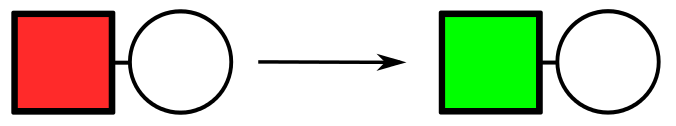
\includegraphics[scale=0.2]{rule_change}}
\end{minipage}

\begin{minipage}[l]{0.1\textwidth}
    \textbf{(c)}
  \end{minipage}
  \begin{minipage}[r]{0.6\textwidth}
    {\hspace*{1.3cm}
\includegraphics[scale=0.2]{rule_diss}}
\end{minipage}
\caption{\textbf{Examples of rules}. Rule \textbf{(a)}: a $\square$ and a $\bigcirc$ can form a complex $\square$--$\bigcirc$ regardless their colors. Rule \textbf{(b)}: a $\square$ is allowed to change it's color from red to green only if it formed a complex with a $\bigcirc$ regardless it's color. Rule \textbf{(c)}: the rule can disassemble the complex only if the $\bigcirc$ is yellow.}
\label{rules:fig}
\end{center}
\end{figure}

The mapping of a rule on a solution can be seen as a particular moment, when the objects in the solution have just the conformation suitable for the rule and therefore the rule can be applied. However, since the distribution of objects is random, we can assume a sequence of objects needed for rule (if there are such objects) is always available.

Moreover, the mapping can be seen as assigning particular objects from the solution to objects on the left-hand-side of the rule. The rule application can be seen as changing the mapped objects to new objects according to the right-hand-side of the rule (i.e., particular objects are assigned to the right-hand-side). As a by-product, we obtain an instance of the rule -- a reaction (see Fig.~\ref{map-apply:fig}). This is how we construct the set of reactions $A$ in the LTS $\mathcal{L}$.

\begin{figure}
\begin{center}
\begin{minipage}[l]{0.1\textwidth}
    \textbf{(a)}
  \end{minipage}
  \begin{minipage}[r]{0.6\textwidth}
    {\hspace*{1.3cm}
\includegraphics[scale=0.2]{rule_complex}}
\end{minipage}

\begin{minipage}[l]{0.1\textwidth}
    \textbf{(b)}
  \end{minipage}
  \begin{minipage}[r]{0.6\textwidth}
    {\hspace*{1.3cm}
\includegraphics[scale=0.2]{rule_complex_mapped}}
\end{minipage}

\begin{minipage}[l]{0.1\textwidth}
    \textbf{(c)}
  \end{minipage}
  \begin{minipage}[r]{0.6\textwidth}
    {\hspace*{1.3cm}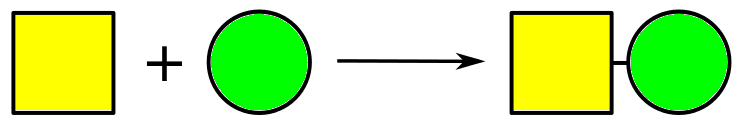
\includegraphics[scale=0.2]{rule_reaction}}
\end{minipage}
\caption{\textbf{Example of a map-apply action}. As a solution, we use solution \textit{(a)} from Fig.~\ref{solutions:fig}. \textbf{(a)} Rule can be mapped on a $\square$ and a $\bigcirc$ regardless their colors and form a complex $\square$--$\bigcirc$.  \textbf{(b)} Let's choose yellow $\square$ and green $\bigcirc$ from our solution. The rule was mapped on choosen objects and they were assigned to the left-hand-side of the rule. \textbf{(c)} The rule was applied and new object (yellow-green complex $\square$--$\bigcirc$) was created. We obtained the reaction describing the particular action which has just happened.}
\label{map-apply:fig}
\end{center}
\end{figure}

Since this kind of graphical representation is not very suitable for describing the processes and for transferring them.. ???, in next chapter(s) we define a formal language which is built on principles described in this chapter.

\section{Rule-based languages}

briefly explain main languages (kappa, BNGL, Recon, Chromar)

show main differences

\section{History of Biochemical Space}

from informal BCS through definition by embedding to Kappa

why not good enough

\chapter{Problem formulation}

why we need something new

what was wrong before

highlight we choose indirect definition via reactions - "practical definition"

\chapter{Formal definition}

\section{Syntax}

\section{Semantics}

\section{Syntactic extensions}

\chapter{Analysis}

\section{Dynamic analysis}

such as simulation, model checking (reachability)

\section{Static analysis}

well... some algorithms are done, but this part need improvement

\chapter{Implementation}

BCSgen, part of a project, several iterations

before it was done via Kappa, what was quite slow (direct rule-based semantics)

explain why it was slow (no abstraction)

\chapter{Case study}

BCS used on ecyano

key features

who practical examples of defined objects

\chapter{Conclusions}

\printbibliography

\end{document}
